\chapter{\texorpdfstring{\Z}{Z} binning}
\label{app:Zbinning}
Note: This section currently has 8 TeV information and has not been updated

We bin events with an OSSF pair depending on whether the pair invariant mass is in the \Z window, or below/above. In case of ambiguity, we need to pick a specific pair. We compare two methods:
\begin{enumerate}
	\item We take the pair whose invariant mass is closest to the \Z mass.
	\item We take the pair closest to the \Z mass, with the additional condition that pairs above the \Z window are not considered if there is a pair below the \Z window (thus shifting events from high-\Z to low-\Z).
\end{enumerate}
Fig.~\ref{fig:app:Zbinning} shows that there is little difference to both approaches. We decide to take the second approach to achieve a more separative categorization of background, especially around the high end of the \Z window.

\begin{figure}
\begin{center}
	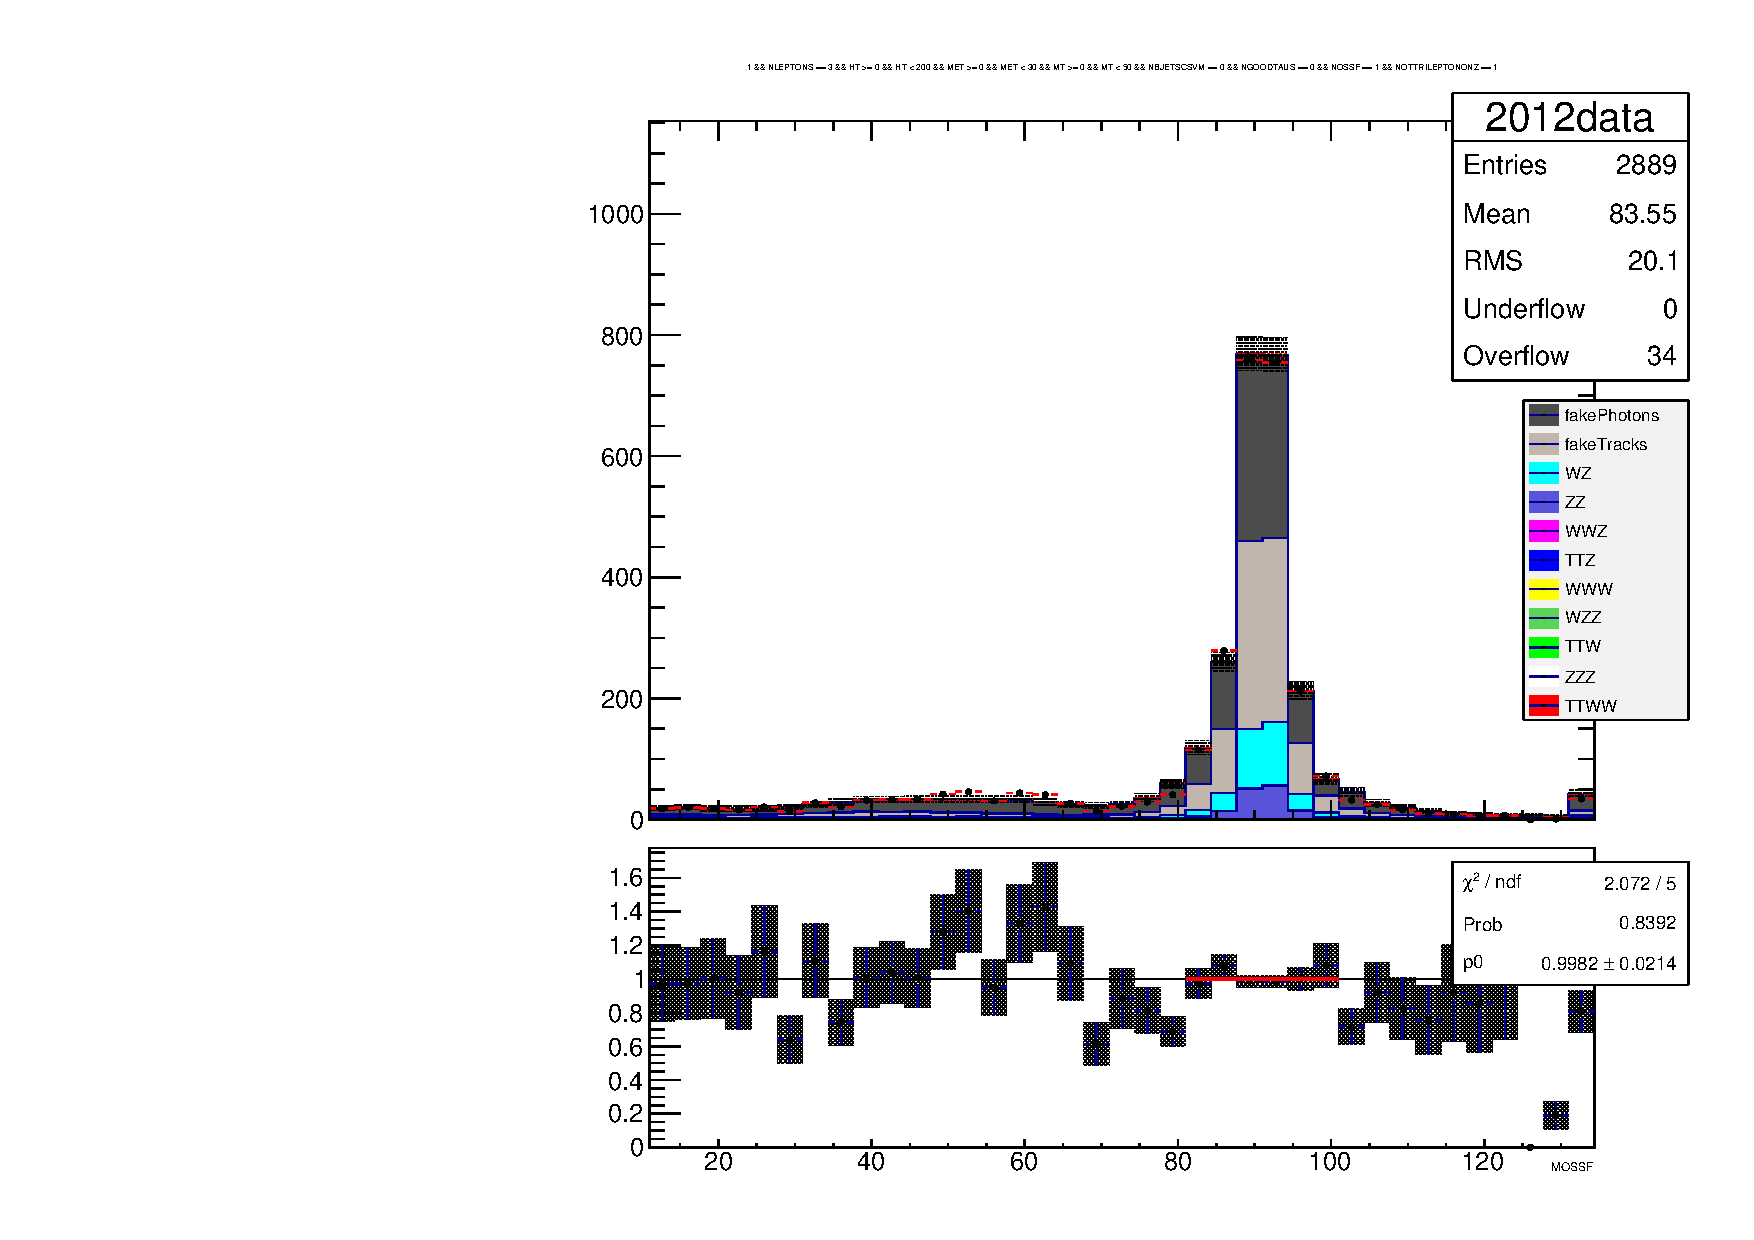
\includegraphics[width=.5\textwidth]{Appendix/Z_NOTTRILEPTONONZ_oldMOSSF}%
	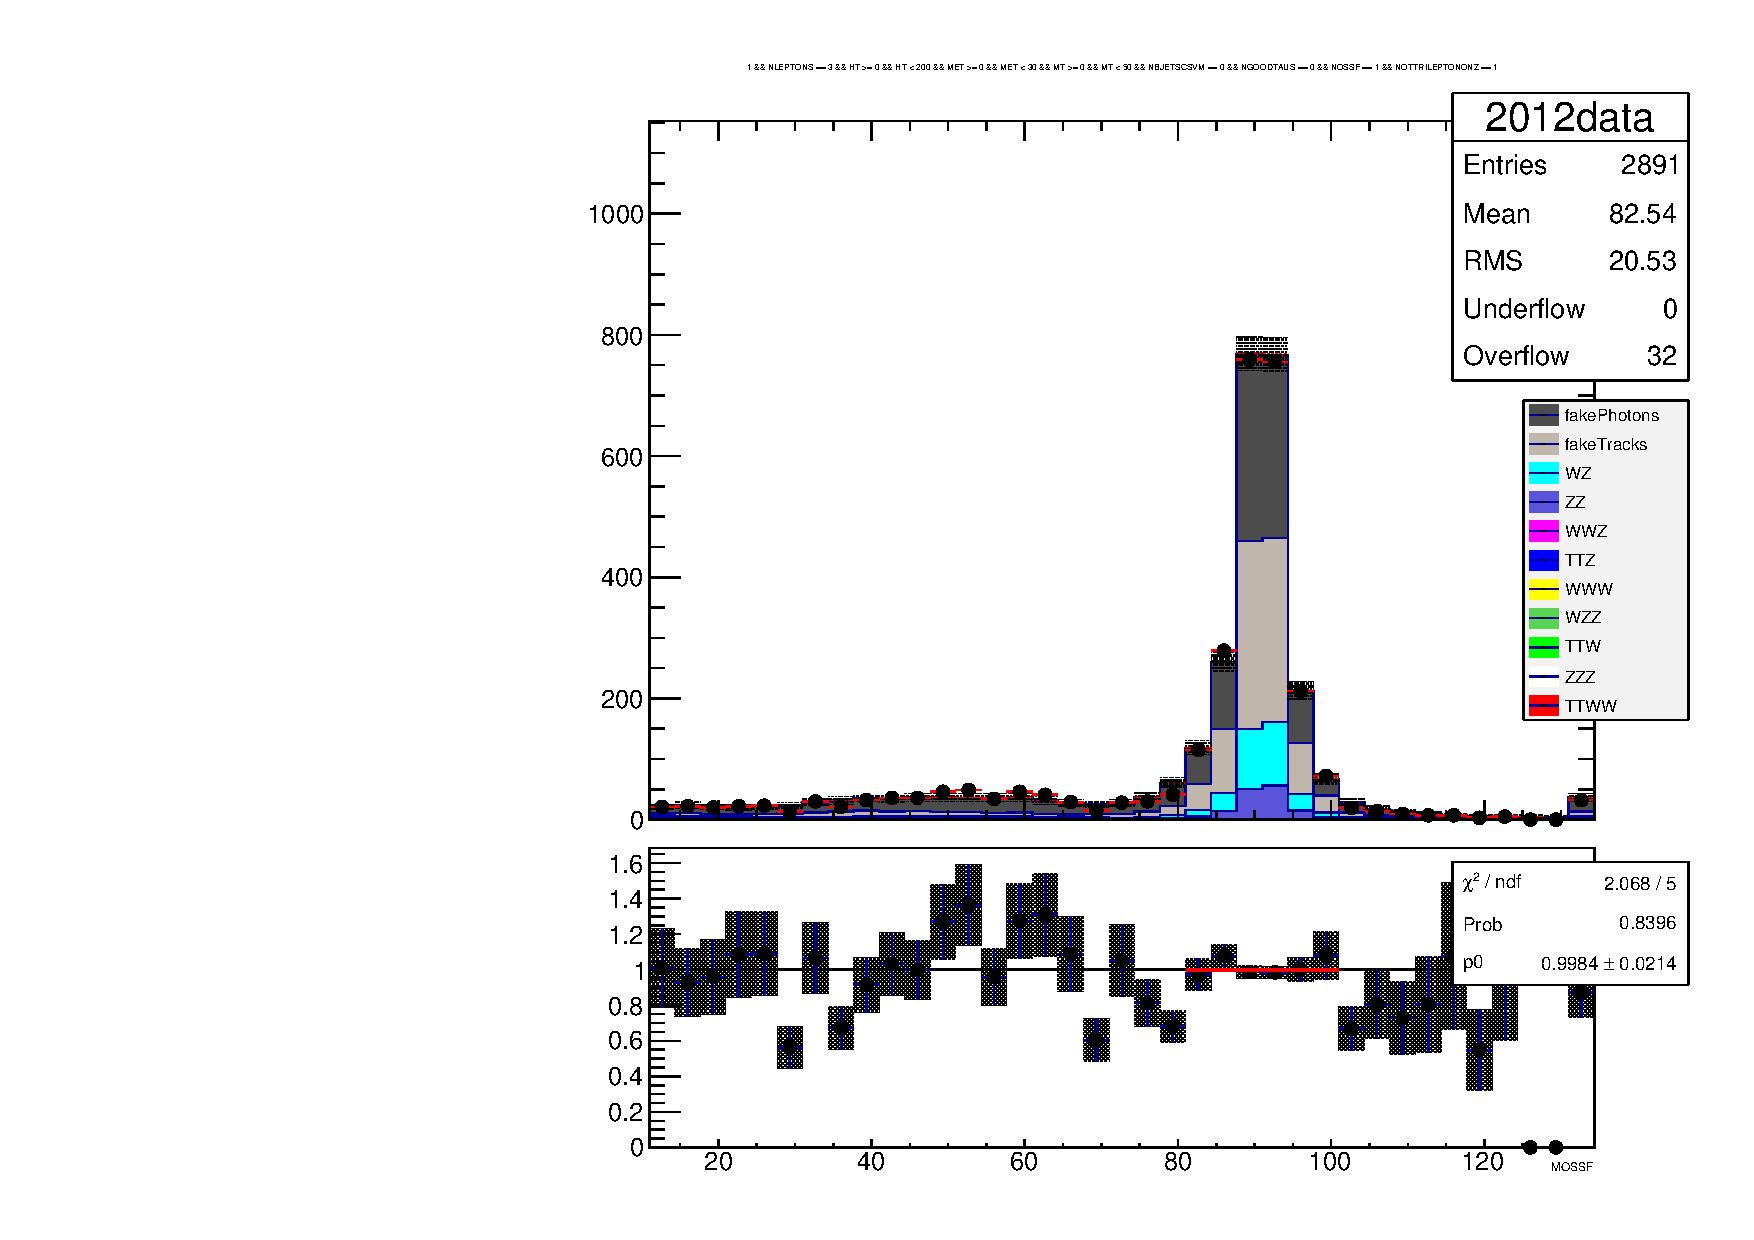
\includegraphics[width=.5\textwidth]{Appendix/Z_NOTTRILEPTONONZ_MOSSF}
	\caption{$m_{\ell\ell}$ distribution in in the dilepton fake region (off-\Z, trilepton events with $m_{\ell\ell\ell}$ on \Z have been vetoed). \enskip left)~method 1 \enskip right)~method 2
	\label{fig:app:Zbinning}}
\end{center}
\end{figure}
